\documentclass[utf8,usehyperref,12pt]{G7-32}
\usepackage[T2A]{fontenc}
\usepackage[utf8]{inputenc} %% ваша любимая кодировка здесь
\usepackage[russian]{babel} %% это необходимо для включения переносов
\usepackage{float}
\usepackage{textcase} 
\usepackage{lastpage}
\usepackage[dvips]{graphicx}
\graphicspath{{pictures/}}
\DeclareGraphicsRule{*}{eps}{*}{}
\TableInChaper % таблицы будут нумероваться в пределах раздела
\PicInChaper   % рисунки будут нумероваться в пределах раздела
\setlength\GostItemGap{2mm}% для красоты можно менять от~0мм

% Определяем заголовки для титульной страницы
\NirOrgLongName{
Министерство общего и профессионального образования РФ

\MakeUppercase{Санкт-петербургский государственный университет информационных технологий, механики и оптики}
}
%\NirBoss{Научный руководитель}{И.И.Упырёв} %% Заказчик, утверждающийНИР
\NirManager{Научный руководитель}{Р.~В.~Иванов} 

\NirYear{2010}%% если нужно поменять год отчёта; если закомментировано, ставитсятекущий год
\NirTown{г. Санкт-Петербург,} %% город, в котором написан отчёт
% по проекту \No8550: 

% \NirIsAnnotacion{АННОТАЦИОННЫЙ } %% Раскомментируйте, если это аннотационный
%отчёт

\NirUdk{УДК \No 2123132123}
\NirGosNo{Регистрационный \No 123123}

%\NirStage{Этап \No 1.1}{промежуточный}{<<Обзор современного состояния торсионных
%наногенераторов>>} %%% Этап НИР: {номер этапа}{вид отчёта - промежуточный или
%заключительный}{название этапа}

\bibliographystyle{unsrt} %Стиль библиографических ссылок БибТеХа

%%%%%%%<------------- НАЧАЛО ДОКУМЕНТА
\begin{document}
\usefont{T2A}{ftm}{m}{} %%% Использование шрифтов Т2 для возможности скопировать
%текст из PDF-файлов.

\frontmatter %%% <-- это выключает нумерацию ВСЕГО; здесь начинаются
%ненумерованные главы типа Исполнители, Обозначения и~прочее

\NirTitle{\textbf{<<Выпускная квалификационная работа>>}}
%%% Название НИР и~генерация титульного листа


\Executors %% Список исполнителей здесь
%% это рисует линию размера 3мм и~толщиной 0.1 пункт
\begin{longtable}{p{0.35\linewidth}p{0.2\linewidth}p{0.35\linewidth}}
Научный руководитель, 	&		&	\\
Р.В.~Иванов	&\rule{1\linewidth}{0.1pt}	&  \\ \vspace{1cm}

Выполнил  &		&	\\
Н.В.~Назаренко, & \rule{1\linewidth}{0.1pt}& \\
\end{longtable}

\Referat %% Реферат отчёта, не~более 1 страницы
Отчёт \pageref{LastPage}~c. 4~рис., 3~табл.

\MakeUppercase{Linux, хранилилище, webdav}



\tableofcontents

%\NormRefs % Нормативные ссылки 
\Defines % Необходимые определения 
СУБД -
FUSE -


\Introduction

placeholder

\mainmatter %% это включает нумерацию глав и~секций в документе ниже

\chapter{Глава 1. Обзор и техническое задание}

\section{Обзор особенностей заказчика}
\subsection{Организационная структура}
Санкт-петербургский городской дворец творчества юных(СпбГДТЮ) обладает большой и сложной организационной структурой, для каждого 
элемента которого, характерен свой вид деятельности. Рассмотрим организацию с точки зрения двух аспектов: территориального
и структурного.

\begin{figure}[ht]
   \centering%центрируем картинку
   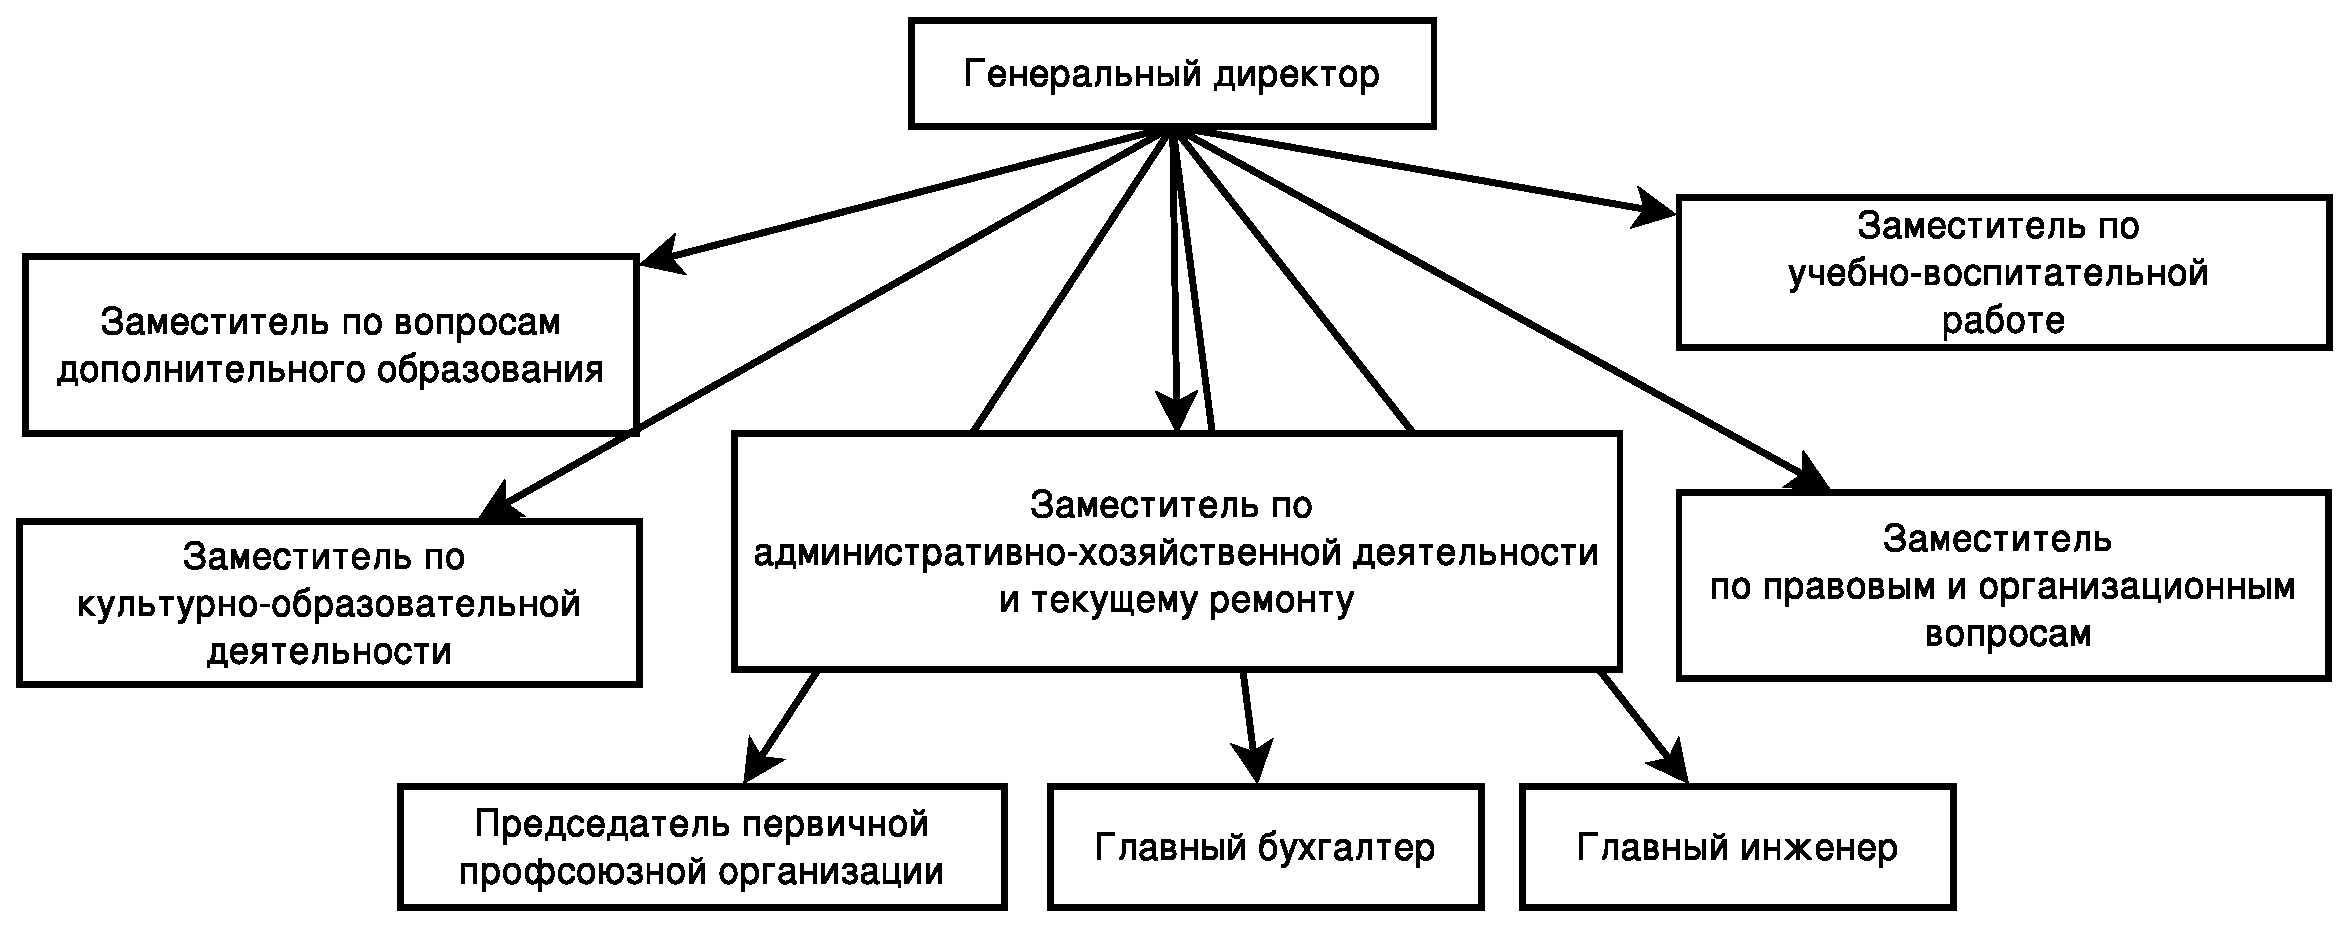
\includegraphics[height=160mm, width=0.8\textwidth, clip, keepaspectratio]{pictures/management_structure.eps}
   \caption{Структура управления организацией}\label{fig:fig_management_struct}
 \end{figure}

Территориальная распределенность обусловленна тем, что Дворец творчества юных расположен в центре города, на его территории находиться множество отдельных корпусов, а также ему принадлежит довольно большой участок земли на Крестовском острове и ЗЦДЮТ «Зеркальный». Доступ пользователей к глобальным и локальным информационным ресурсам обеспечивается подключениями по выделенной линии
(2 мб/с), по оптоволокну (1000 мб/с) и прямыми подключениями к узлу (100 мб/с). Сеть рассчитана на большое количество пользователей ИТ-инфраструктурой (более
15 000 компьютеров). Среди них: работники дворца; педагоги; управляющий персонал;  персонал, отвечающий за сервисную деятельность; учащиеся. Сложность управленческой структуры организации определяется большим штатом сотрудников и широким спектром исполняемых функций. Главным руководителем является генеральный директор, которому подчиняются различные подразделения такие как: финансовый, хозяйственный, учебно-воспитательный и другие сектора.

\begin{figure}[ht]
   \centering%центрируем картинку
   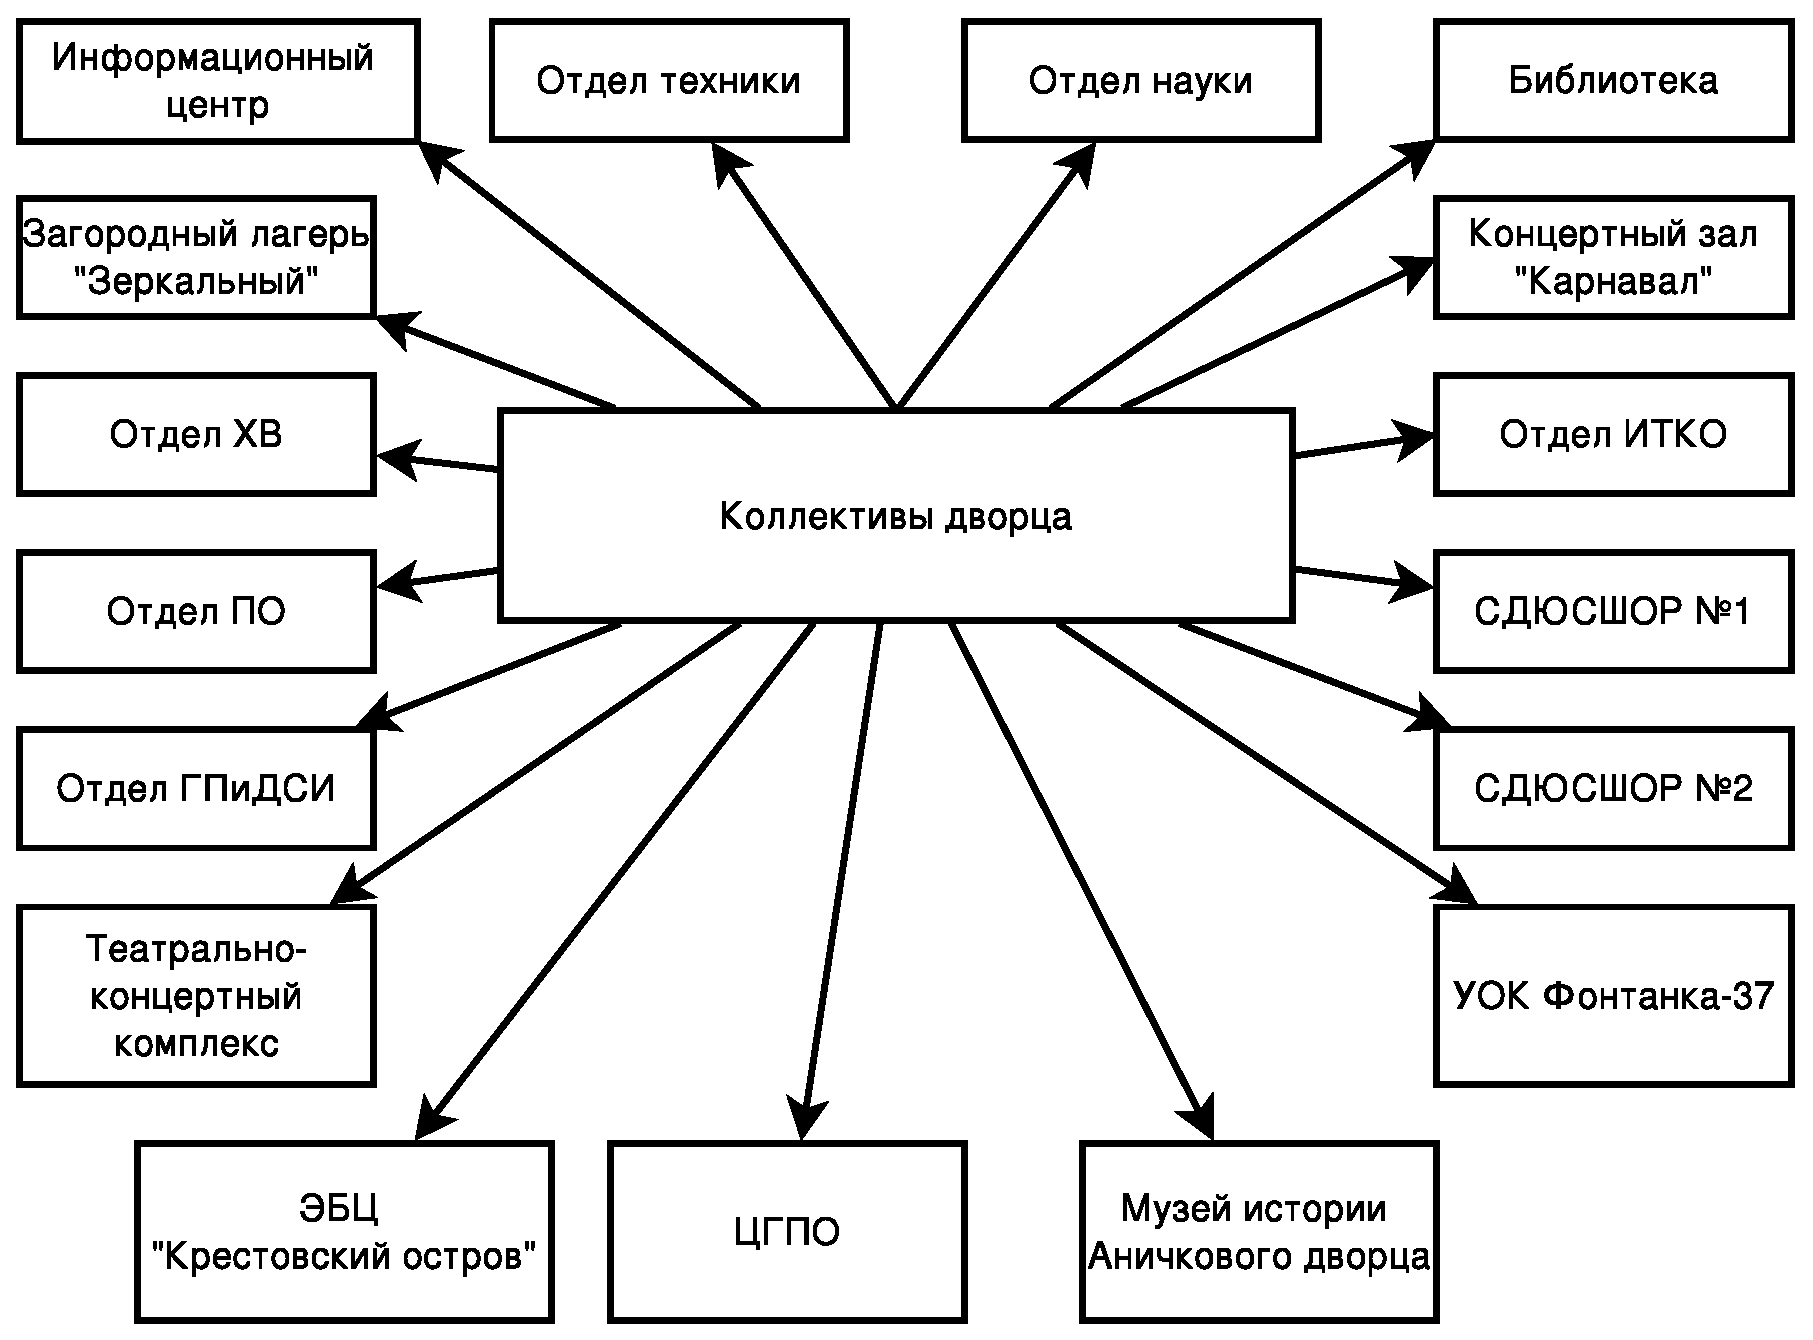
\includegraphics[height=160mm, width=0.8\textwidth, clip, keepaspectratio]{pictures/org_struct.eps}
   \caption{Структура подразделений}\label{fig:org_structure}
 \end{figure}

Сотрудники дворца разделены на коллективы или отделы, отвечающие за определенный вид деятельности(рисунок \ref{fig:org_structure}).
Каждый отдел в свою очередь имеет большое количество своих подразделений. У каждого коллектива или отдела есть свой директор, один или несколько заместителей и большое количество сотрудников.


\begin{itemize}
\item Отдел ХВ – отдел художественного воспитания
\item Отдел ПО – отдел предшкольного  образования
\item Отдел ГПиДСИ – отдел гуманитарных программ и детских социальных инициатив
\item Отдел ИТКО – отдел информационных технологий и компьютерного обеспечения
\item СДЮС школа №1 – специализированная детско-юношеская спортивная школа №1
\item СДЮС школа № – специализированная детско-юношеская спортивная школа №2
\item УОК <<фонтанка-37>> – учебно-оздоровительный комплекс <<фонтанка-37>>
\item ЭБЦ <<крестовский остров>> – эколого-биологический центр <<крестовский остров>>
\item ЦГПО – центр городских предметных олимпиад.
\end{itemize}

Основной функцией дворца является оказание образовательных и воспитательных услуг, которые оказывают учебные коллективы, осуществляющие свою деятельность под управлением методических подразделений самого Дворца
и управляющих организаций МОиН города. Кроме непосредственно обучения сотрудники  составляют различные учебные программы, рабочие планы, отчеты, разрабатывают учебно-методические пособия.
Обеспечением текущей деятельности дворца, в аспекте поддержания в надлежащем состоянии оборудования, коммуникаций занимаются сервисные подразделения Дворца. Схема должностей СПБГТЮ представлена на рисунке \ref{fig:fig_management_struct}.

\subsection{Задачи требующие инфраструктурного сопровождения}\label{ssect:tasks_infra}
Основной функцией дворца является оказание образовательных и воспитательных услуг, предоставление которых оказывают учебные коллективы, осуществляющие свою деятельность под управлением методических подразделений самого Дворца
и управляющих организаций МОиН города. Кроме непосредственно обучения сотрудники составляют различные учебные программы, рабочие планы, отчеты, разрабатывают учебно-методические пособия. 

Для обеспечения работы сотрудников требуется система сетевого хранения файлов по подразделениям с возможностью разделения прав доступа сотрудников. Такое разделение необходимо для того, чтобы . Для разных подразделений это могут быть различные виды файлов: изображения, документы в различных форматах, аудио или видео информация и так далее. Подразделениям необходима возможность выкладывать файлы в общий доступ.

\subsection{Ограничения накладываемые на информационное сопровождение}\label{ssect:restrict_infra}
Поскольку организация осуществляет переход на свободное программное обеспечение, то требуется использование исключительно свободных программных продуктов для реализации системы хрпнения файлов. В проекте используются только компоненты распространяющиеся под свободными лицензиями, одобренными OSI(Open Software Initiative). Решение должно функционировать в операционной системе GNU/Linux и быть независимым от ОС установленной на рабочем месте пользователя.

У педагогов в следствии недостатка времени и иногда отсутствия желания осваивать новый продукт могут возникнуть трудности при переходе на новую информационную систему. С другой стороны, педагоги – люди, которые умеют учиться, что является неоспоримым плюсом для более быстрого перехода на новую систему.

Кроме того, многие педагоги работают не только во Дворце, но и дома, где зачастую используется другое программное обеспечение, в большинстве случаев проприетарное. Следовательно, необходимо предоставить возможность доступа к служебной информации, методическим и др. материалам, необходимым для обеспечения профессиональной деятельности без привязки к определённым операционным системам.

Управленческий аппарат почти весь состоит из людей далёких от информационный технологий. У таких сотрудников нет желания менять устоявшийся бизнес-процесс, поэтому их приходиться заставлять переучиваться, используя административный ресурс, что накладывает жёсткие ограничения на сложность использования системы хранения файлов.

%Сервисные сотрудники обладают большим количеством свободного времени,
%но у них отсутствует желание работать, трудиться, им свойственна лень, поэтому им не хочется учиться, но процесс обучения у них происходит быстрее за счёт имеющихся знаний.

Во Дворце ежедневного находится большое количество сотрудников, выполняющих свои непосредственные обязанности, поэтому функционирование Дворца является непрерывным процессом, поэтому его не только не следует приостанавливать,
а категорически не рекомендуется это делать.

Таким образом система сетевого доступа к файлам должна быть максимально простой с точки зрения пользователя, использовать стандартизованные решения, реализации которых есть под все популярные операционные системы и быть открытым программным обеспечением.

\subsection{Предположительные архитектурные решения и задачи информационной системы}
Исходя из положений раздела~\ref{ssect:tasks_infra} задачей хранилища данных является хранение файлов пользователей, дерева каталогов, информации о пользователях и их правах доступа. В процессе работы, пользователи будут использовать большое количество различных форматов файлов, поэтому представление файла в системе хранения должно быть максимально обобщённым. 

Система ориентирована на пользователей с различным уровнем знакомства с информационными технологиями(раздел~\ref{ssect:restrict_infra}). Для минимизации риска утери данных при случайном удалении или перезаписи файлов требуется реализовать хранение истории версий таким образом, чтобы пользователь мог получить доступ к удалённому файлу или одной из предыдущих доступных версий. В то же время, для уменьшения обьёма данных хранящихся на жестком диске хранилища, требуется возможность окончательного удаления предыдущих версий файлов по прошествии определённого срока администратором системы.

Для осуществления контроля за действиями пользователей и поиска ошибок в работе системы требуется сохранять информацию о действиях пользователей в системе с момента входа в систему. Для поиска проблемы необходимо знать какие действия выполнял пользователь в указанный момент времени и были ли ему разрешены данные действия правами доступа на тот момент.

Таким образом требуется:
\begin{itemize}
\item осуществление разделения пользователей по ролям доступа
\item предоставление удобного доступа пользователя к файлам и директориям, на которые ему были установлены права доступа.
\item хранение предыдущих версий файлов с возможностью их последующего удаления
\item ведение журнала активности пользователей
\end{itemize}

Исходя из требований к системе, предлагается трёхзвенная архитектура: Клиент -- сервер приложений -- хранилище данных. Такая архитектура позволяет разделить логику работы клиент-серверной части и хранения файлов в хранилище данных. 

\section{Обзор аналогов}
\subsection{Samba}

Samba — программа, которая позволяет обращаться к сетевым дискам на различных операционных системах по протоколу SMB/CIFS. 
Имеет клиентскую и серверную части. Является свободным программным обеспечением, выпущена под лицензией GPL. Такая система удобна в использовании, предоставляет удобный доступ клиенту к файлам, не требует предварительной передачи на жёсткий диск пользователя. Минусами данного варианта реализации является ориентированность на работу в локальной сети, отсутствие версионности хранящихся файлов.

<<<<<<< HEAD
%\subsection{FTP с разделением прав}
=======
\subsection{FTP с разделением прав}
FTP (англ. File Transfer Protocol — протокол передачи файлов) — протокол, предназначенный для передачи файлов в компьютерных сетях. FTP позволяет подключаться к серверам FTP, просматривать содержимое каталогов и загружать файлы с сервера или на сервер; кроме того, возможен режим передачи файлов между серверами. FTP является одним из старейших прикладных протоколов, появившимся задолго до HTTP, в 1971 году.
>>>>>>> 307b81c63a23c948808b9fc518cea4bc88496526

Данное решение сложно в настройке, использовании. У этого решения отсутствует возможность 
удалённой работы с файлами. Файлы требуется сначала загрузить на локальный диск, внести 
изменения и после этого загрузить обратно на сервер. При этом не сохраняется предыдущая версия файла. При использовании такого решения, сложно получать информацию об изменениях прав доступа, модификациях файлов и дерева каталогов. Версионность доступа реализуется с только с помощью версионных ФС. При использовании такого решения приходится либо использовать встроенные средства авторизации, которые в большинстве своём не обладают достаточной гибкостью, либо создавать системных пользователей на сервере, что при неправильной настройке политик доступа может представлять собой уязхвимое место в системе.

\subsection{Системы управления версиями}
Система управления версиями — программное обеспечение для облегчения работы с изменяющейся информацией. Система управления версиями позволяет хранить несколько версий одного и того же документа, при необходимости, возвращаться к более ранним версиям, определять, кто и когда сделал то или иное изменение и многое другое.

Системы контроля версий такие как: git, svn, cvs; требуют определённой подготовки от пользователя. Это решение требует от пользователя ручного получения файлов из хранилища и помещения их обратно. Исходя из причин по которым создавались такие системы, невозможно ограничить глубину сохранения версий файлов, что при использовании не-текстовых данных приводит к быстрому разрастанию хранилища файлов.

Решение на основе git является наиболее безопасным, поскольку все данные передаются через шифрованное соединение, а аутентификация пользователя производится на основе криптографических ключей.

\subsection{Системы электронного документооборота}
Система документооборота, система электронного документооборота (СЭД) — автоматизированная многопользовательская система, сопровождающая процесс управления работой иерархической организации с целью обеспечения выполнения этой организацией своих функций. При этом предполагается, что процесс управления опирается на человеко-читаемые документы, содержащие в слабоформализованной форме инструкции для сотрудников организации, необходимые к исполнению.

Такие системы оориентированы на управление бизнес-процессами и оперируют понятием документа. Организовать в такой системе совместную работу над разнородными материалами, такими как методические пособия сложно, поскольку зачастую это может быть мультимедийная информация к обработке и хранению которой СЭД не приспособлены.

\section{Формализация техического задания}
\subsection{Платформа}
Исходя из ограничений описанных в разделе~\ref{ssect:restrict_infra} требуется использование исключительно свободного ПО для реализации системы хранения файлов. 
\subsection{Средства разработки}

\subsection{Функциональные ограничения}

Требуется ведение журнала активности пользователей, включающего в себя информацию о следующих действиях: 
\begin{itemize}
\item дату и время входа/выхода пользователя
\item создание файла
\item модификация файла
\item удаление файла
\item установка блокировки на файл
\item снятие блокировки с файла
\end{itemize}

Требуется предоставить удобный доступ пользователя к файлам и директориям, на которые ему были установлены права доступа такие как: чтение, запись, удаление файлов и каталогов.

Требуется разработать инструмент позволяющий:	
\begin{itemize}
\item получать информацию об изменениях произошедших с последнего входа пользователя в систему	
\item выполнять аутентификацию пользователя по логину/паролю	
\item выполнять подключение рабочей области пользователя в дерево каталогов
\end{itemize}

Необходимо осуществлять разделение пользователей по следующим ролям:	
\begin{itemize}
\item Пользователь 	в соответствие со своими правами имеет 	доступ к файлам и каталогам подразделения и к общим каталогам. Имеет доступ к предыдущим версиям своих файлов на чтение. 		
\item Администратор подразделения может назначать права 	доступа для сотрудников подразделения, создавать и удалять каталоги в каталоге подразделения. Имеет доступ на чтение к предыдущим версиям файлов подразделения	
\item Администратор создает и удаляет учётные записи пользователей, записи подразделений, назначает права доступа, имеет полный 	доступ к дереву каталогов, имеет полный 	доступ к предыдущим версиям файлов.
\end{itemize}

\chapter{Глава 2. Проектирование}
\section{Системные архитектурные решения}
\subsection{Распределение задач между компонентами}
Бизнес логика реализуется на сервере приложений, в рамках которой обеспечивается:
\begin{itemize}
\item авторизация пользователей, 
\item предоставление требуемых файлов и каталогов для работы в соответствие с правами доступа, 
\item блокировка используемых файлов 
\item получение обновлённой версии с возможным получением предыдущих версий файла.
\item запись информации о действиях пользователей в рамках системы
 \end{itemize}
 
Клиентская часть реализует сетевой доступ к файлам находящимся в хранилище, посредством WebDAV протокола. Задачами клиентской части являются:
\begin{itemize}
\item запрос учётных данных пользователя
\item реализация представления файловой системы и подключение её к дереву каталогов пользователя
\item реализацию протокола общения между клиентской частью и сервером приложений
\item передача файлов пользователя серверу приложений
\item получение запрошенных файлов с сервера приложений
\end{itemize}

Хранилище данных решает задачу хранения пользовательских данных, файлов, дерева каталогов и вспомогательных сущностей.
%\subsection{Описание задач решаемых отдельными компонентами}
\subsection{Описание интерфейсов между компонентами}

\section{Архитектура программы}
\subsection{Архитектура БД}

В проекте используется технология объектно-реляционного отображения, позволяющая работать с записями в БД, как с объектами языка программирования. Такой подход позволяет представить БД как абстрактное хранилище объектов и не задумываться над деталями конкретной реализации БД.

Для хранения данных может использоваться любая реляционная СУБД, которая поддерживается выбранной библиотекой для объектно-реляционного отображения.

\begin{figure}[ht]
   \centering%центрируем картинку
   \includegraphics[height=160mm, width=0.8\textwidth, clip, keepaspectratio]{pictures/DB.eps}
   \caption{Схема БД}\label{fig:db_scheme}
 \end{figure}

Основные сущности используемые в системе показаны на рисунке \ref{fig:db_scheme}. В БД хранится информация о пользователях, группах, правах доступа, хранящихся файлах их содержимом и версиях.
 
\subsection{Архитектура клиентской части}

Клиентская часть реализует доступ к файловому хранилищу как к подкаталогу в дереве файлов пользователя. Это достигается использованием средств, которые позволяют предоставить POSIX интерфейс к сетевому хранилищу данных.

\begin{figure}[ht]
   \centering%центрируем картинку
   \includegraphics[height=160mm, width=0.8\textwidth, clip, keepaspectratio]{pictures/client_sequencs.eps}
   \caption{Схема взаимодействия клиента с сервером приложений}\label{fig:client_sequence}
 \end{figure}

На диаграмме последовательностей (рисунок \ref{fig:client_sequence}) показаны события происходящие в процессе работы пользователя с файловой системой. В работе пользователя выделяются три основных этапа: монтирование, изменение объектов файловой системы и отмонтирование системы. 

При монтировании ФС, у пользователя запрашивают его логин/пароль для работы в системе, после этого сервер приложений проверяет правильность введённых данных и аутентифицирует его и возвращает содержимое корневой директории пользователя.

При изменениии файла происходит блокировка ресурса на сервере приложений. Запись данных пользователем идёт в локальный кэш, который через некоторое время отправляется на сервер приложений. Использование кеширования позволяет уменьшить количество версий файлов, особенно для приложений в которых используется автосохранение файлов.

При отмонтировании происходит оттравка данных из кеша клиентской части на сервер приложений и отключение от сервера приложений.

\subsection{Архитектура сервера приложений}

Сервер приложений используется для обработки запросов пользователей и подготовкой полученных файлов к сохранению в хранилище. Сервер приложений состоит из многопоточного обработчика запросов пользователей, обработчика аутентификации и авторизации пользователей и обработчика davfs протокола используемого для связи с клиентским приложением.

\begin{figure}[ht]
   \centering%центрируем картинку
   \includegraphics[height=160mm, width=0.8\textwidth, clip, keepaspectratio]{pictures/davstorage.eps}
   \caption{Диаграмма значимых классов проекта}\label{fig:davstorage}
 \end{figure}
 
 Диаграмма классов системы, без реализации WebDAV и http-сервера представлена на рисунке \ref{fig:davstorage}. Система постоена на принципе независимости от реализации хранения файлов и информации о пользователях, что позволяет реализовать своё хранилище данных, реализующее интерфейс для WebDAV протокола.

\section{Проектирование инфраструктуры}
\subsection{Оценка требований к серверу}
\subsection{Оценка требований к рабочему месту пользователя}
\subsection{Оценка требований к пропускной способности канала}

\chapter{Глава 3. Реализация}
\section{Особенности реализации БД}
\section{Особенности реализации инструмента администрирования}
\section{Особенности реализации клиентской части}
Клиентская часть состоит из модуля к FUSE, утилит монтирования и графического интерфейса для утилит монтирования для упрощения работы пользователям. 

--- Картинка с пояснением, что такое FUSE
\section{Особенности тестирования и отладки}
\section{План внедрения и отладки}
\subsection{Организационные мероприятия}
\subsection{Технические мероприятия}
\subsection{Мероприятия сопровождения}

\chapter{Глава 4. Экономическая часть}
\chapter{Глава 5. Безопасность}

\Conclusion
заключение

\end{document}